\chapter{Building a data set for Comparative Argument Mining}
\section{Common Crawl Text Corpus}
The raw data used for the creation of the dataset was derived from CommonCrawl. CommonCrawl is a non-profit organisation which crawls the web and releases the data and metadata with a loose license. This master thesis uses the crawl data from DATE. Furthermore, the data was processed: HTML was stripped out, and the content was splitted into sentences using X. To make the data maintainable, the sentences where imported into an ElasticSearch index. The index has a size of 1.1tb and contains 3,288,963,864 unique sentences.

To get an idea how many sentences in the index may be comparative, searches with cue words was performed. The query \texttt{better OR easier OR faster OR nicer OR wiser OR cooler OR decent OR safer OR superior OR solid OR teriffic OR worse OR harder OR slower OR poorly OR uglier OR poorer OR lousy OR nastier OR inferior OR mediocre} yields 55,627,400 results, the more specific query \texttt{is better than} yields 428,932 results.

Those numbers indicate that the index contains enough comparative sentences to create machine learning data set.

Lesen \cite{Panchenko:2017aa}

\section{Prestudy}
Previous to the main study, a pre-study was conducted to assess the quality of the annotation guidelines, the approach of sentence generation and the task itself.


\subsection{Data Selection and Preprocessing}
\label{sec:prestudy-processing}
To obtain comparative sentences from the ElasticSearch index, Query \ref{lst:es-query-a} was used. The sentence must contain two comparable objects (like "Apple" and "Pear") and at least one cue word. Presence of the cue words \enquote{better}, \enquote{worse}, \enquote{superior} and \enquote{inferior} should increase the probability of the sentence to be comparative. Because the pre-study was conducted on a small data set (1000 sentences) the list of cue words is rather short. In this way, the amount of noisy sentences should be reduced.
However, not all comparisons will contain one of the cue words, so 25\% of the sentences sentences where obtained without the cue words.


\begin{lstlisting}[label=lst:es-query-a,breaklines=true,postbreak=\mbox{\textcolor{red}{$\hookrightarrow$}\space}]
  {
        "query" : {
            "bool": {
                "must": [
                    {
                        "query_string": {
                            "default_field" : "text",
                            "query" :  "(better OR worse OR superior OR inferior) AND \"<OBJECT_A>\" AND \"<OBJECT_B>\""
                        }
                    }
                ]
            }
        }
    }
\end{lstlisting}



Ten hand-selected object pairs were used (see table \ref{tbl:prestudy-objects}). The pairs were chosen to cover a wide range of different objects, which was expected to yield differently phrased arguments. The pairs where chosen to obtain a wide range of different objects, which will lead to different comparisons. Some sentences contain programming- and computer specific terms, so a need for this knowledge was expressed.
\begin{table}[h]
\centering
\caption{Objects of the Annotation Prestudy}
\label{tbl:prestudy-objects}
\begin{tabular}{@{}llrrr@{}}
\toprule
First Object & Second Object      & \# Sentences & Mean Length  & Std                             \\ \midrule
Ruby    & Python    & 109    & 235.94 & 48.70 \\
BMW    & Mercedes    & 107 & 246.66 & 47.68\\
USA & Europe & 106 & 241.90 & 50.80\\
Beef & Chicken & 106 & 241.76 & 52.66  \\
Android & iPhone    &   104 & 211.08  & 36.46 \\
Cat & Dog      &     104 & 216.65 & 43.01 \\ 
Football & Baseball   &  104 & 230.19  & 42.29 \\ 
Wine & Beer  & 104 & 228.07 & 49.20 \\
Car & Bicycle & 103 & 242.54 & 47.89\\
Summer & Winter &  103 & 211.65 & 36.16\\  \midrule 
 \multicolumn{2}{c}{Average} & 1050 & 230.76 & 47.41\\ 
\bottomrule  
                               
\end{tabular}
\end{table}

The retrieved sentences where further filtered and processed. Each sentence must be between 15 and 200 characters long and must not contain more than seven punctuation characters. In this ways, lists are removed. Also, the sentence must contain each of the two objects exactly once.


\subsection{Task}
The annotators where asked to assign one of the four following classes to each sentence.\newline

\emph{BETTER}: This class should be used if the sentence indicates that object A is better in any way than object B.

\emph{WORSE}: Same as \emph{BETTER}, but the sentence must indicate that object A is worse than object B.

\emph{UNCLEAR}: If the sentence contains an argument, but it is not between A and B, this class should be used.

\emph{NO\_COMP}: All other sentences fall into this category.\newline

In a test first step, 112 sentences where obtained with the procedure described in chapter \ref{sec:prestudy-processing}.
Twelve sentences were used as test sentences to filter out people who did not read the annotation guidelines.

The sentences were preprocessed: the first object was replaced by OBJECT\_A, the second by OBJECT\_B. Examples are shown in table \ref{tbl:pre1s}. The removal was done so that the annotators can concentrate on the comparative structure of the sentence and are not biased by the objects.


% Beispielsätze PreStudy 1. Teil
\begin{table}[h]
\centering
\caption{Sentences for the first pre-study}
\label{tbl:pre1s}
\begin{tabular}{{p{12cm}p{3cm}}}
\toprule
Sentence            & Expected Class \\ \midrule
This is potentially useful for OBJECT\_A, PHP, JS and OBJECT\_B.                                 & NO\_COMP       \\
Also keep in mind that OBJECT\_A blends will give you worse mileage than OBJECT\_B & WORSE      \\ 
Snowboarding during OBJECT\_A is a lot better than during OBJECT\_B. & BETTER \\
\bottomrule
\end{tabular}
\end{table}



This test step delivered valuable insights. First, the amount of test sentences was to small. Users might see the same test sentence twice. Second, the phrasing of the annotation guidelines was to confusing, especially the distinction between NO\_COMP and UNCLEAR.
Third, the complete removal of the original objects also removed parts of the sense of the sentences, which can make the annotation process harder.\newline

The actual pre-study was conducted with 200 sentences and 51 test sentences. Furthermore, the preprocessing was changed. Instead of removing the original objects, :[OBJECT\_A] was appended to the first object, :[OBJECT\_B] to the second object. Also, each object was highlighted in a different color. Example sentences are shown in table \ref{tbl:pre2s}. In this way, the annotators could quickly see the objects of interest while the sense of the sentence remains intact.
% Beispielsätze PreStudy 2. Teil
\begin{table}[h]
\centering
\caption{Sentences for the second pre-study}
\label{tbl:pre2s}
\begin{tabular}{{p{12cm}p{3cm}}}
\toprule
Sentence                                                                                                           & Expected Class \\ \midrule
I'd go with \textbf{{\color[HTML]{9A14B2} python:{[}OBJECT\_A{]}}} or \textbf{{\color[HTML]{6CB219}ruby:{[}OBJECT\_B{]}}}.                                 & NO\_COMP       \\
I prefer \textbf{{\color[HTML]{9A14B2}ruby:{[}OBJECT\_A{]}}} over \textbf{{\color[HTML]{6CB219}python:{[}OBJECT\_B{]}}} on windows.                                              & BETTER         \\
I've tried \textbf{{\color[HTML]{9A14B2}python:{[}OBJECT\_A{]}}}, and can see why people like it, but \textbf{{\color[HTML]{6CB219}ruby:{[}OBJECT\_B{]}}} suits my style better. & WORSE          \\
i think this car is a far better deal than the \textbf{{\color[HTML]{9A14B2}bmw{:[OBJECT\_A]}}} 5 series or \textbf{{\color[HTML]{6CB219}mercedes:[OBJECT\_B]}} 320e.                                                                                                                &        UNCLEAR        \\ \bottomrule
\end{tabular}
\end{table}

\label{sec:annotation-guidelines}
\subsection{Results}
Each sentence was annotated by three annotators. Figure \ref{pre:dist} shows the class distribution.

\begin{figure}[h]
\centering
\caption{Class Distribution in the prestudy}
\label{pre:dist}
\begin{tikzpicture}
\pie [rotate=180, text = legend, color= {cgray, cgreen, cred, cblue}]
    {59.76/NO\_COMP,
    23.11/BETTER,
    9.16/WORSE,
    7.97/UNCLEAR }
\end{tikzpicture}
\end{figure}


%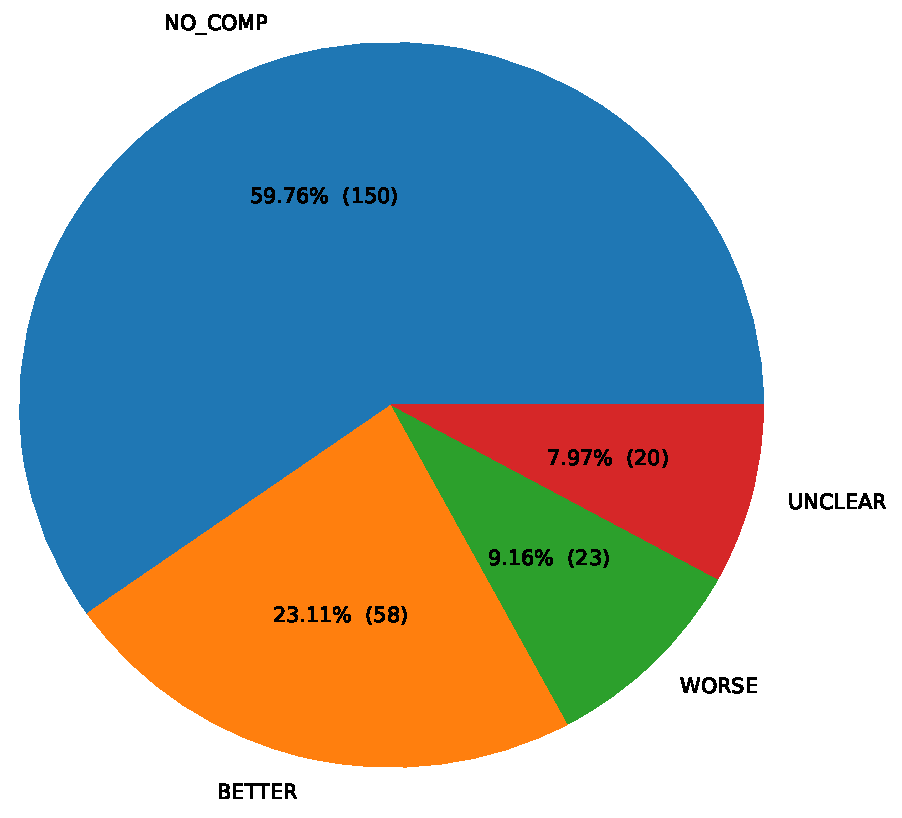
\includegraphics[scale=0.6]{images/prestudy/label_distribution.pdf}


Crowdflower has a trust value for each annotator. This trust value and the number of votes per class gives a value of confidence for each label.\footnote{How the confidence is calculated in detail can be found at https://success.crowdflower.com/hc/en-us/articles/201855939-How-to-Calculate-a-Confidence-Score (Last checked: 19.12.2017)}


As presented in figure \ref{pre:conf}, a majority (151) of the labelings has a confidence greater or equal to 0.9, and 15 sentences a confidence below 0.6; the mean is 0.86. Detailed numbers on the confidence are shown in table \ref{pre:conf-table}

\begin{figure}
\centering
\caption{Confidence histogram}
\label{pre:conf}
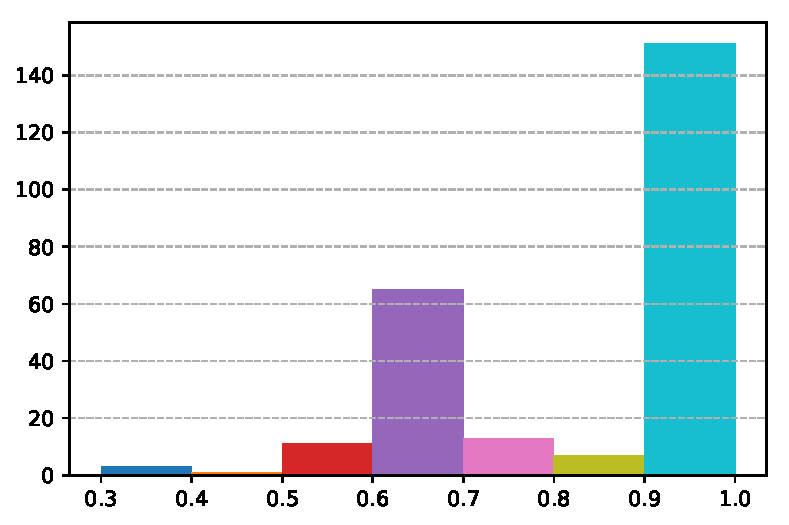
\includegraphics[scale=0.6]{images/prestudy/confidence.pdf}
\end{figure}


\begin{figure}[h]
\centering
\caption{Confidence}
\begin{tabular}{@{}ll@{}}
\toprule
Type & Value  \\ \midrule
Average Confidence & 0.86 \\
Standard Derivation & 0.17 \\
Lowest Confidence & 0.35\\
Highest Confidence & 1.00\\
25th percentile average & 0.67\\
50th percentile average & 1.00\\
\bottomrule
\label{pre:conf-table}
\end{tabular}
\end{figure}





The most difficult sentence is with a confidence of 0.35 for the class \emph{WORSE} was
\begin{quote}
Google shouldn't have mandated an inferior map app on the iphone:[OBJECT\_A] (as opposed to android:[OBJECT\_B]).
\end{quote}

It was labelled as \emph{BETTER} (trust: 0.72), \emph{WORSE} (trust: 0.85) and \emph{NO\_COMP} (trust: 0.82). The class \emph{WRONG} is correct here, as the object \enquote{iphone} is inferior to \enquote{android} on the aspect of \enquote{map app}.

The following sentence was assigned to \emph{BETTER} (0.37 confidence), although it should belong to \emph{UNCLEAR}.
\begin{quote}
Not to mention that the iphone:[OBJECT\_A] and android:[OBJECT\_B] phones deliver a far superior user experience overall
\end{quote}
However, the annotator for \emph{UNCLEAR} only had 0.87 trust, while the one for \emph{BETTER} had 1 (third one was \emph{NO\_COMP} with 0.82 trust).\newline

All things considered, the result of the prestudy is satisfactory. The annotators agreed in the majority of decisions. 



\section{Main Study}
